\chapter{Analysis}
	
	
	\section{Verification of a problem}\label{sec:verification}
		\subsection{Why a problem?}
		
		\subsection{Who says so?}
		
		\subsection{Why does it matter?}
		
		\subsection{Elder people's approach to technology}
		In most cases old people will not search for technology in general as a solution, when they seek to do actions they usually would not be able to, due to their age limitations. The age limitation in some cases lead to loss of mobility, and therefore a decrease in life quality according to studies\todo{Needs reference}. \\
		
		\subsection{Interviews}

		The target group had been defined as "people who go to gardening centers", and as specific as that is (which is very little), we needed to know more about the target group. Do this end, unstructured interviews were conducted at a garden center with its customers. This way we would get a better understanding of both the target group and the context the product would be used in. Furthermore, we also had the option of observing the target group in a natural environment, performing the task that we aim to help them with. Also during this time we had access to staff at the center and could inquire as to what their thought would work \\
		
		% when and where
		% what does location and time mean for the data
		List of questions for target group
		\begin{itemize}
			\item[-] Have you ever used a garden designer?
			\item[-] What was your experience?
			\item[-] What are you planning to buy?
			\item[-] What are you plan/thoughts for when you buy a new plant?
			\item[-] What do you consider when you buy a new item for your garden?
			\item[-] How often do you make major changes to your garden?
			\item[-] For which reasons did you decide to purchase this item?
			\item[-] What was the latest item you bought that you were not satisfied with?
			\item[-] Do you have a garden?
			\item[-] How did you start the design process?
			\item[-] What tools did you use, if any?
			\item[-] When did you make changes to your garden?
			\item[-] What big changes would you like to make?
			\item[-] Are you retired?
			\item[-] If you had all the time in the world, what would you change about your garden?
			\item[-] Do you enter the garden center with a budget in mind?
			\item[-] Why are you here? \\
		\end{itemize}
		
		List of questions for experts \\
		Target group questions:
		\begin{itemize}
			\item[-] Which people usually adresses you?
			\item[-] What is the most usual demography?
			\item[-] Do people need designing for all or just parts of their garden?
			\item[-] Who makes the 3D visualisation of the garden? Is it something you create internally in the company, or does it come from outside cooperators? 
			\item[-] How does this process function?
			\item[-] Do people take the offer on 3D visualisation of their garden?
			\item[-] What about development over time? Does it mean that growth can be followed year by year, or does it concern seasons?
			\item[-] Is it something people make use of? \\
		\end{itemize}
		
		Technology questions:
		\begin{itemize}
			\item[-] How do you think a Virtual Reality experience in the 3D environment would be received?
			\item[-] If a customer could design their own garden in a gardening center and instantly visualise it in Virtual Reality, do you think it would be a popular choice? \\
		\end{itemize}
		
		Design questions:
		\begin{itemize}
			\item[-] How large of a garden area do you usually work with?
			\item[-] What plants are trending at the moment?
			\item[-] What is a popular garden style?
		\end{itemize}

		\subsubsection{Demographic information}
		\begin{itemize}
			\item[-] Sex
			\item[-] Age
			\item[-] Job
			\item[-] Gift
			\item[-] Level of education
		\end{itemize}

	\section{Context}
		
	\section{Target group}\label{sec:targetGroup}
		\subsection{Who are the target }
		
	\section{Technologies}\label{sec:technologies}
		\subsection{Virtual Reality}
			The earliest attempts at a VR experience was in the 1950s\cite{VRS} by Morton Heilig who made the Sensorama\ref{fig:sensorama}; an arcade-style theater cabinet, that featured stereo speakers, stereoscopic 3D display, smell generators, fans and a vibrating chair.
			\begin{figure}[h]
				\centering
				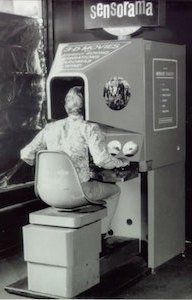
\includegraphics[width=0.4\linewidth]{figure/Analysis/sensorama2}
				\caption{The Sensorama made by Morton Heilig in the 1950s}
				\label{fig:sensorama}
			\end{figure}
			There were a couple of short movies made for the Sensorama, but these were all produced and edited by Morton Heilig himself. The whole setup was stationary, and didn't feature any Head Mounted Display (HMD), so the user had to sit in the vibrating chair and look straight at the display for the duration of the movie.
		\subsection{Image Processing}
			\subsubsection{Color detection}
			
			\subsubsection{Edge detection}
			
			\subsubsection{Blob detection}
			
			\subsubsection{Object recognition}

    \section{State of the art}\label{sec:SOTA}
		\subsection{Other vr applications}
		
		\subsection{Some sketching tools maybe}
		
		\subsection{Reactivision applications for reference}
		
		\subsection{AR garden things maybe}
		